\documentclass[11pt, a4paper]{article}
\usepackage[a4paper, margin = 0.7in]{geometry}
\usepackage{graphicx}
\usepackage{amsmath}
\usepackage{listings}
\usepackage{url}

\title{EE2703 Assignment 8 : The Digital Fourier Transform}
\author{Aman Kumar EE19B066}
\date{May 20, 2021}

\begin{document}

\maketitle

\section{Introduction}
In this assignment we will learn about DFT and FFT. We will be plotting the spectrum of many functions. One of those is also going to be \textbf{not} bandlimited. Suppose $f[n]$ are the samples of some function $f(t)$, then we define the Z transform as:
\begin{equation*}
    F(z) = \sum_{n = -\infty}^{\infty}f[n]z^{-n}
\end{equation*}
Replacing $z$ with $e^{j\theta}$ we get:
\begin{equation*}
    F(e^{j\theta}) = \sum_{n = -\infty}^{\infty}f[n]e^{-jn\theta}
\end{equation*}
$F(e^{j\theta})$ is called the Digital Spectrum of the samples $f[n]$. It is also called the DTFT of $f[n]$. When $f[n]$ is discrete and aperiodic, $F(e^{j\theta})$ is continuous and periodic. If $f[n]$ is a periodic sequence of samples, with a period $N$. Then the DTFT of the sequence is also a periodic sequence $F[k]$ with the same period $N$. So we have
\begin{equation}
    F[k] = \sum_{n=0}^{N-1}f[n]exp(-2\pi \frac{nk}{N} j) = \sum_{n=0}^{N-1}f[n]W^{}nk
\end{equation}
\begin{equation}
    f[n] = \frac{1}{N}\sum_{k=0}^{N-1}F[k]W^{-nk}
\end{equation}
The values $F[k]$ are what remains of the Digital Spectrum $F(e^{j\theta})$. We can consider them as the values of $F(e^{j\theta})$ for $\theta = 2\pi k/N$. What this means is that the DFT is a sampled version of the DTFT, which is the
digital version of the analog Fourier Transform.
\section{The Assignment}
There are two commands in Python, one to compute the forward fourier transform and the other to compute the inverse transform. They are:
\begin{verbatim}
numpy.fft.fft()
numpy.fft.ifft()
\end{verbatim}
We will be using these to get the transforms and then plotting the spectrums.
    \subsection{The function \texttt{plot\_spectrum()}}
    I have made this function to plot the spectrums of different functions it is  such that the plots are highly customizable. The phase in the plots is in degrees. \textbf{Note :} while plotting phase spectrum, it plots phase only when magnitude is greater than $10^{-3}$. Its argumnents are:
    \begin{enumerate}
        \item \textbf{y} : function
        \item \textbf{Nsamples} : number of samples
        \item \textbf{Title} : title of the plot
        \item \textbf{n\_fig} : number of the figure
        \item \textbf{Xlim} : x-axis range in the plot
        \item \textbf{tick\_size} : size of font in ticks
        \item \textbf{x\_ticks} : ticks along x-axis
        \item \textbf{y\_ticks} : ticks along y-axis
    \end{enumerate}
    \begin{verbatim}
def plot_spectrum(y,Nsamples,Title,n_fig,Xlim,tick_size,x_ticks=None,y_ticks=None):
    Y = p.fftshift(p.fft(y))/Nsamples       #Calculating the tranform
    w = p.linspace(-64,64,Nsamples+1)       #The frequency axis of the plot
    w = w[:-1]

    p.figure(n_fig - 1)
    p.subplot(2,1,1)                        #First subplot : Magnitude
    p.plot(w,abs(Y))
    p.xlim(Xlim)
    p.yticks(y_ticks,size=tick_size)
    p.xticks(x_ticks,size=tick_size)
    p.ylabel(r"$|Y|$",size=11)
    p.title(Title)
    p.grid(True)

    p.subplot(2,1,2)                        #Second subplot : Phase
    ii = p.where(abs(Y) > 1e-3)             #Finding indexes where |Y| > 1e-3
    p.plot(w[ii],p.angle(Y[ii])*(180/p.pi),'ro',markersize=4)
    p.xlim(Xlim)
    p.xticks(x_ticks,size=tick_size)
    p.yticks(p.arange(-180,185,90),size=10)
    p.ylabel(r"Phase of $Y$",size=11)
    p.xlabel(r"$k$",size=11)
    p.grid(True)
    p.show()
    \end{verbatim}
    \subsection{Spectrum of $sin(5x)$}
    This function is known to us. We know that
    \begin{equation*}
        y = sin(5x) = \frac{e^{j5x} - e^{-j5x}}{2j}
    \end{equation*}
    So the expected spectrum is
    \begin{equation*}
        Y(\omega) = \frac{1}{2j} [\delta(\omega - 5) - \delta(\omega + 5)]
    \end{equation*}
        \subsubsection{First Attempt}
        In the first attempt we did not use \texttt{fftshift()} and also $0$ (or $2\pi$) point is repeating. Python code for plotting:
        \begin{verbatim}
#Example 1 sin(5t) "Bad"
x = p.linspace(0,2*p.pi,128)           #x-range fron 0 to 2pi
y = p.sin(5*x)
Y = p.fft(y)                           #Calculating the transform of y

p.figure(0)
p.subplot(2,1,1)                       #Subplot 1 : Magnitude
p.plot(abs(Y))
p.xticks(p.arange(0,130,5),size=5)
p.ylabel(r"$|Y|$",size=11)
p.title(r"Spectrum of $\sin(5t)$")
p.grid(True)

p.subplot(2,1,2)                       #Subplot 2 : Phase
p.plot(p.angle(Y)*(180/p.pi))          #I am plotting the phase in degrees
p.xticks(p.arange(0,130,5),size=5)
p.yticks(p.arange(-180,185,90),size=10)
p.ylabel(r"Phase of $Y$",size=11)
p.xlabel(r"$k$",size=11)
p.grid(True)
#p.savefig("Figure 1.png")
p.show()
        \end{verbatim}
        \begin{figure}[!h]
            \centering
            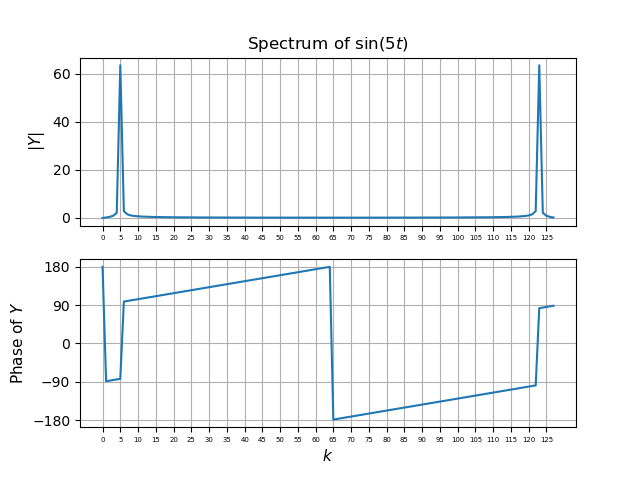
\includegraphics[scale = 0.7]{Figure 1.png}
            \caption{Spectrum of $sin(5t)$ (Bad)}
            \label{fig:Figure 1}
        \end{figure}
        From the plot we observe:
        \begin{itemize}
            \item Power is not zero for frequencies other than the peaks.
            \item We got peaks but not where we expected. Also, the height of the peaks is $64$ whereas it should have been $0.5$.
            \item The phase at the peaks is near $90^{\circ}$ but not exact.
        \end{itemize}
        \subsubsection{Second attempt}
        This time we use \texttt{fftshift()} to shift the $\pi$ to $2\pi$ portion to the left as it represents negative frequency. And we also make $x$ stop just before $2\pi$ so that point is not repeated. We divide by $N$ to get the height of the peaks right.
        \begin{verbatim}
x = p.linspace(0,2*p.pi,129)      #129 samples from 0 to 2pi
x = x[:-1]                        #Dropping the last sample to make it 128(2^7)
y = p.sin(5*x)                    #sampling freq = 128/2pi
Title = "Spectrum of $\sin(5t)$"
plot_spectrum(y,128,Title,2,[-10,10],10,p.arange(-10,11,5),p.arange(0,0.51,0.25))
        \end{verbatim}
        \begin{figure}[!h]
            \centering
            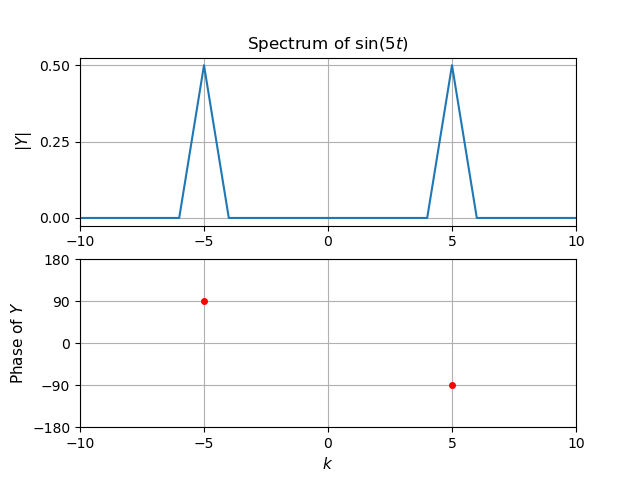
\includegraphics[scale = 0.66]{Figure 2.png}
            \caption{Spectrum of $sin(5t)$}
            \label{fig:Figure 2}
        \end{figure}
    \subsection{Spectrum of $(1+0.1cos(t))cos(10t)$}
    \begin{equation*}
        y = cos(10t) + 0.1cos(t)cos(10t) = cos(10t) + 0.05(cos(11t) +cos(9t))
    \end{equation*}
    \begin{equation*}
        y = 0.5(e^{j10t} + e^{-j10t}) + 0.025(e^{j11t} + e^{j9t} + e^{-j11t} + e^{-j9t})
    \end{equation*}
        \subsubsection{First attempt}
        We try to get the spectrum using the same parameters we used above to get the spectrum of $sin(5t)$.
        \begin{figure}[!h]
            \centering
            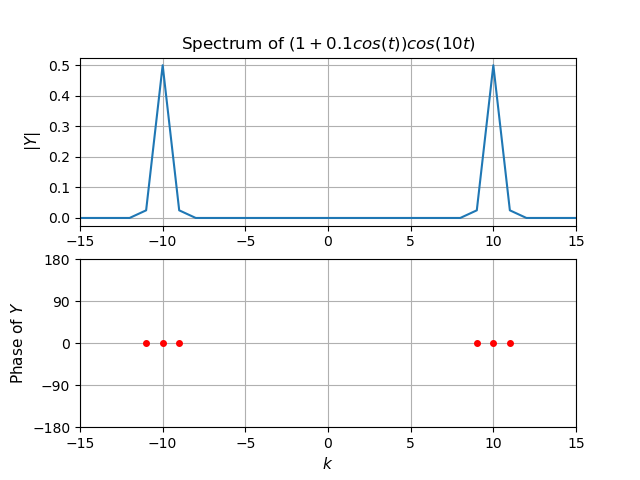
\includegraphics[scale = 0.66]{Figure 3.png}
            \caption{Spectrum of $(1+0.1cos(t))cos(10t)$ (Bad)}
            \label{fig:Figure 3}
        \end{figure}
        
        Instead of getting three different peaks, we are getting a single broad peak. To fix this we must stretch the time axis while keeing the sampling frequency same. Thus we change $x$-range from $[0,2\pi]$ to $[-4\pi,4\pi]$ and also increase $N$ from $128$ to $512$ to keep the sampling frequency same.
        \begin{verbatim}
x = p.linspace(-4*p.pi,4*p.pi,513)  #513 samples from -4pi to 4pi
x = x[:-1]                          #Dropping the last sample to make it 512(2^9)
y = (1+0.1*p.cos(x))*p.cos(10*x)
plot_spectrum(y,512,Title,4,[-15,15],8,p.arange(-15,16,5),p.arange(0,0.51,0.1))
        \end{verbatim}
        \begin{figure}[!h]
            \centering
            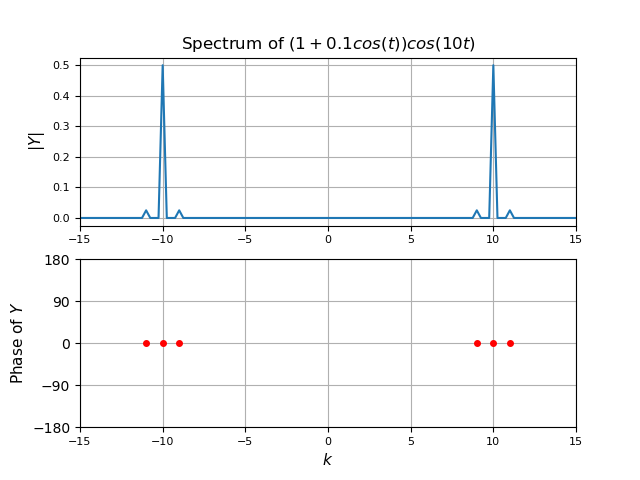
\includegraphics[scale = .7]{Figure 4.png}
            \caption{Spectrum of $(1+0.1cos(t))cos(10t)$ with bigger time range}
            \label{fig:Figure 4}
        \end{figure}
    \subsection{Spectrum of $sin^3(t)$ and $cos^3(t)$}
    We know that
    \begin{equation*}
        y_1 = sin^3(t) = \frac{3sin(t) - sin(3t)}{4} = \frac{3}{8j}(e^{jt} - e^{-jt}) - \frac{1}{8j}(e^{j3t} - e^{-j3t})
    \end{equation*}
    \begin{equation*}
        Y_1(\omega) = \frac{3}{8j}(\delta(\omega-1) - \delta(\omega+1)) - \frac{1}{8j}(\delta(\omega-3) - \delta(\omega+3))
    \end{equation*}
    and
    \begin{equation*}
        y_2 = cos^3(t) = \frac{3cos(t) + cos(3t)}{4} = \frac{3}{8}(e^{jt} + e^{-jt}) + \frac{1}{8}(e^{j3t} + e^{-j3t})
    \end{equation*}
    \begin{equation*}
        Y_2(\omega) = \frac{3}{8}(\delta(\omega-1) + \delta(\omega+1)) - \frac{1}{8}(\delta(\omega-3) + \delta(\omega+3))        
    \end{equation*}
    
    Using the same parameters as we used in the previous section, we plot the spectrums of $sin^3(t)$ and $cos^3(t)$ in Figure $5$ and Figure $6$ respectively. The python code snippet for plotting:
    \begin{verbatim}
y = (p.sin(x))**3          #Defining the function
Title = "Spectrum of $sin^3(t)$"
plot_spectrum(y,512,Title,5,[-5,5],10,p.arange(-4,5,1),p.arange(0,0.51,0.1))

y = (p.cos(x))**3          #Defining the function
Title = "Spectrum of $cos^3(t)$"
plot_spectrum(y,512,Title,6,[-5,5],10,p.arange(-4,5,1),p.arange(0,0.51,0.1))
    \end{verbatim}
    \begin{figure}[!h]
        \centering
        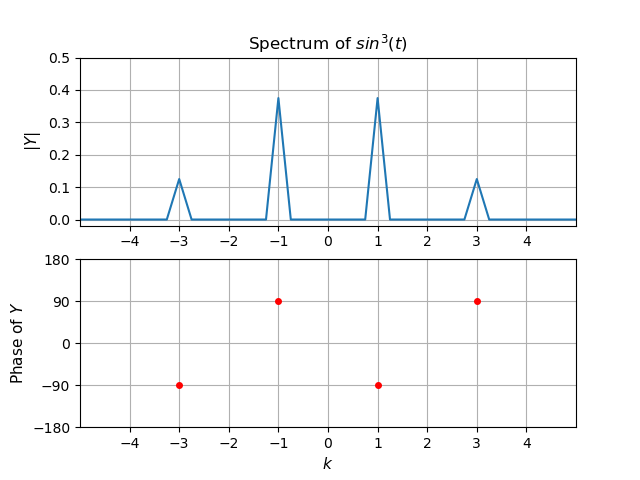
\includegraphics[scale = 0.7]{Figure 5.png}
        \caption{Spectrum of $sin^3(t)$}
        \label{fig:Figure 5}
    \end{figure}
    The heights of the peaks and their phases are all as expected for the spectrum of both these functions.
    \begin{figure}[!h]
        \centering
        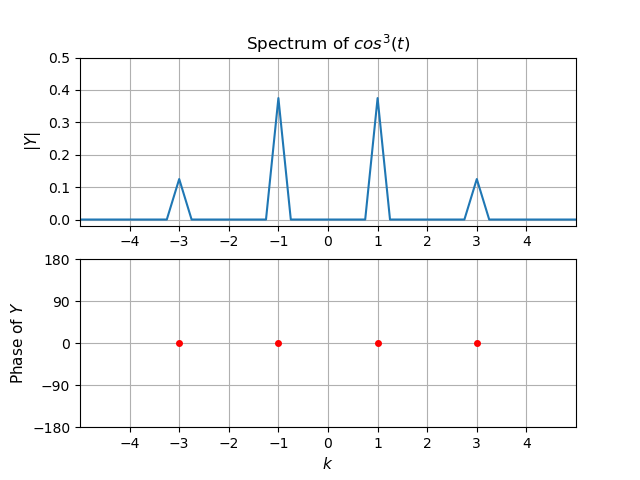
\includegraphics[scale = 0.7]{Figure 6.png}
        \caption{Spectrum of $cos^3(t)$}
        \label{fig:Figure 6}
    \end{figure}
    \subsection{Spectrum of $cos(20t +5cos(t))$}
    We have to
    \begin{itemize}
        \item Plot the magnitude and phase spectrum.
        \item Plot phase only when magnitude is greater than $10^{-3}$.
        \item Discuss about the spectrum obtained.
    \end{itemize}
    Python code for finding and plotting the spectrum of $cos(20t +5cos(t))$is given below :
    \begin{verbatim}
y = p.cos(20*x + 5*p.cos(x))
Title = "Spectrum of $cos(20t +5cos(t))$"
plot_spectrum(y,512,Title,7,[-35,35],8,p.arange(-35,36,5))
    \end{verbatim}
    \begin{figure}[!h]
        \centering
        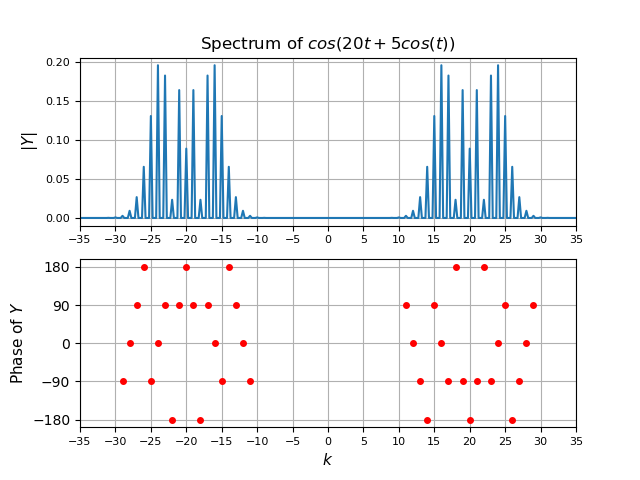
\includegraphics[scale = 0.7]{Figure 7.png}
        \caption{Spectrum of $cos(20t +5cos(t))$}
        \label{fig:Figure 7}
    \end{figure}
    \begin{itemize}
        \item The plot is Phase modulated since phase of the signal, varying proportionally to amplitude of the message signal, is $\omega = 20$ and infinite side band frequencies which are produced by $5cos(t)$, since $cos(t)$ is infinitely long signal. But the strength of the side band frequencies either decays or is very small as they are away from the center frequency or carrier frequency component as we observe from the plot.
        \item Since the phase is changed continuously with respect to time, the carrier signal can represent either a sine or cosine depending on the phase contribution from $cos(t)$.
    \end{itemize}
    \subsection{Spectrum of a Gaussian : $exp(-t^2/2)$}
    \begin{itemize}
        \item This is \textbf{not} a bandlimited function. We want to get its spectrum accurate upto $6$ digits. For this we try different time ranges and find which time range gives us that accuracy.
        \item The CTFT of a Gaussian is also a Gaussian. For this function it is given by:
            \begin{equation}
                exp(-t^2/2) \longleftrightarrow \frac{1}{\sqrt{2\pi}} exp(-\omega^2/2)
            \end{equation}
        \item Finding the normalising constant for DFT:
            \begin{enumerate}
                \item Window the signal $exp(-t^2/2)$ by rectangular function with gain $1$ and window size $T$ which is equivalent to convolving with $Tsinc(\omega T)$ in frequency domain. So As $T$ is very large the $sinc(\omega T)$ shrinks , we can approximate that as $\delta(\omega)$. So convolving with that we get same thing.
                \item Now we sample the signal with sampling rate $N$, which is equivalent to convolving impulse train in frequency domain.
                \item Finally for DFT we create periodic copies of the windowed sampled signal and make it periodic and then take one period of its Fourier transform i.e. DFT.
                \item For windowing the signal, we will multiply it with the rectangular function
                    \begin{equation*}
                        y(t) = exp(-t^2/2) \times rect(\frac{t}{\tau}) 
                    \end{equation*}
                    \begin{equation*}
                        rect(\frac{t}{\tau}) = 
                        \begin{cases}
                            1 & \lvert{t}\rvert \leq \tau \\
                            0 & elsewhere
                        \end{cases}
                    \end{equation*}
                \item In the frequency domain, this is equivalent to convolution.
                    \begin{equation*}
                    Y(\omega) = \frac{1}{2\pi}(\frac{1}{\sqrt{2\pi}} exp(-\omega^2/2)*\frac{sin(\tau \omega)}{\omega})
                    \end{equation*}
                    \begin{equation*}
                    \lim_{\tau \to \infty} Y(\omega) = \frac{\tau}{2\pi}(\frac{1}{\sqrt{2\pi}} exp(-\omega^2/2)*\delta(\omega))
                    \end{equation*}
                    \begin{equation*}
                    \lim_{\tau \to \infty} Y(\omega) =  \frac{\tau}{2\pi}(\frac{1}{\sqrt{2\pi}} exp(-\omega^2/2))                       
                    \end{equation*}
                \item Now, sampling this signal with a period of $2\pi/T_s$, we will get $Y_s$ (sampled $Y$)
                    \begin{equation*}
                    Y_{s} = \frac{\tau}{2\pi T_s}\frac{1}{\sqrt{2\pi}} exp(-\omega^2/2) \sum_{k = -\infty}^{\infty}\delta(\omega - \frac{2k\pi}{T_s})
                    \end{equation*}
                \item Solving it, we get the multiplication factor $M$ to be
                    \begin{equation}
                    M = \frac{\tau}{2\pi T_s}    
                    \end{equation}
            \end{enumerate}
        \item I have written a function \texttt{best\_T\_N(tolerance)} which finds the time range $T$ and corresponding $N$ with which the error is less than the tolerance ($10^{-6}$ here) passed to it as argument. After finding the appropriate $T$ and $N$, it plots the spectrum of the given Gaussian function along with its expected spectrum.
    \end{itemize}
        \begin{verbatim}
def best_T_N(tolerance):
    T = 2*p.pi                       #Starting value of T is 2pi
    N = 128                          #Starting value of N is 128 = 2^7
    err = tolerance+1                #Intially making error > tolerance
    
    #This loop will stop only when the error becomes less than tolerance. The
    value of T and N, when the loop stops will be the desired values
    while True:
        x = p.linspace(-T/2,T/2,N+1)[:-1]           #x range
        w = p.linspace(-64,64,N+1)[:-1]             #Frequency axis of the plot
        y = Gauss(x)                                #The given Gauss function
        Y = p.fftshift(p.fft(y))*T/(2*p.pi*N)       #Calculating the Transform 
                                                    #for the current T and N
        Yexp = expected_gauss(w)                    #Expected transform
        err = p.mean(abs(abs(Y) - Yexp))            #Finding the mean error 
                                                    #between calculated and 
                                                    #expected transforms
        
        #If mean error is less than the given tolerance then break the loop
        if(err < tolerance):
            break
        T = 2*T                                     #Updating T
        N = 2*N                                     #Updating N
    
    #Plotting the spectrum for the T and N that we got
    p.figure(7)
    p.subplot(2,1,1)                                #Subplot 1 : Magnitude
    p.title(r"Spectrum of $exp(-x^2/2)$")
    p.plot(w,abs(Y),label="Calculated Y",color="gold",lw=2)                  
    p.plot(w,Yexp,label="Expected Y",lw=1,linestyle="dashed",color="black")  
    p.ylabel(r"$|Y|$")
    p.legend()
    p.grid(True)
    p.xlim([-10,10])
    
    #Subplot 2 : Phase.
    #NOTE: I am plotting phase only when magnitude is greater than 1e-3
    p.subplot(2,1,2)
    ii = p.where(abs(Y) > 1e-3)             #Finding indexes where |Y| > 1e-3
    p.plot(w[ii],p.angle(Y[ii])*(180/p.pi),'ro',markersize=4)
    p.xlabel(r"$k$")
    p.ylabel(r"Phase of $Y$")
    p.yticks(p.arange(-180,185,90),size=10)
    p.xlim([-10,10])
    p.grid(True)
    p.show()
        \end{verbatim}
    \begin{figure}[!h]
        \centering
        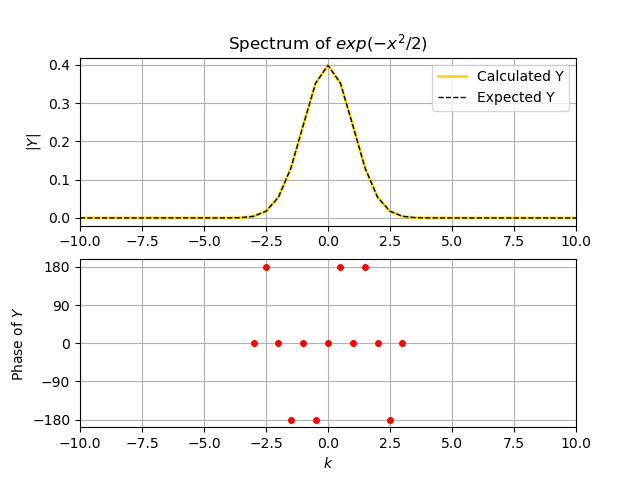
\includegraphics[scale = 0.7]{Figure 8.png}
        \caption{Spectrum of the Gaussian : $exp(-x^2/2)$}
        \label{fig:Figure 8}
    \end{figure}
    The function \texttt{best\_T\_N(tolerance)} also returns the value of $T$, $N$ and mean error from expected transform. These are
    \begin{verbatim}
Best time range : 4.0pi
Corresponding N : 256 samples
Mean error : 2.0757878772955722e-11
    \end{verbatim}
    \begin{itemize}
        \item As we can observe, the magnitude spectrum of $y = exp(-x^2/2)$ almost coincides with the actual Fourier Transform of $y$.
        \item The mean error between calculated and expected magnitude spectrum is approximately just $2.0758^{-11}$.
        \item To overcome the problem of aliasing, we increases the time range $T$ and the number of samples $N$ along with it. We used a \texttt{while} loop for it that will stop only when the mean error is less than the tolerance given.
    \end{itemize}
\section{Conclusion}
In this assignment we
\begin{itemize}
    \item learned how to find and plot the DFT spectrum of various signals. One of them was also a non-periodic, \textbf{not} bandlimited function i.e. $exp(-t^2/2)$.
    \item how to find the normalising factor for DFT of Gaussian functions, to recover analog Fourier trasnform using DFT.
    \item Throughout the assignment we used number of samples belonging to the set $2^k$ and also used FFT instead of DFT which reduces the complexity from $O(n^2)$ to $O(nlog(n))$.
\end{itemize}
 \end{document}
